\documentclass[10pt, xcolor=x11names, compress]{beamer}
%\documentclass[10pt, xcolor=x11names, compress, handout]{beamer}

\usetheme{progressbar}
%\usecolortheme[named=Purple4]{structure}
\progressbaroptions{headline=sections,titlepage=normal,frametitle=normal}

\setbeamertemplate{navigation symbols}{}

\usepackage{iwona} 

\usepackage{alltt}
\usepackage{amsmath,amsfonts, amssymb, amscd}
\usepackage{hyperref}
\usepackage{setspace}
\usepackage{wasysym}
\usepackage{ulem}

\usepackage{calc}
\usepackage[overlay,absolute]{textpos}
\TPGrid[5mm,5mm]{20}{20}

\usetheme{progressbar}
%\usecolortheme[named=Purple4]{structure}
\progressbaroptions{headline=sections,titlepage=normal,frametitle=normal}

\setbeamertemplate{navigation symbols}{}

\usepackage{iwona} 

\usepackage{alltt}
\usepackage{amsmath,amsfonts, amssymb, amscd}
\usepackage{hyperref}
\usepackage{setspace}
\usepackage{wasysym}
\usepackage{ulem}

\usepackage{calc}
\usepackage[overlay,absolute]{textpos}
\TPGrid[5mm,5mm]{20}{20}



\renewcommand{\Re}{\operatorname{Re}}
\renewcommand{\Im}{\operatorname{Im}}
\newcommand{\debye}{\operatorname{debye}}

\newcommand{\chik}{$\chi(k)$}
\newcommand{\chir}{$|\tilde{\chi}(R)|$}


\newcommand{\file}[1]{{\color{Firebrick4}\texttt{`#1'}}}
\newcommand{\multiple}{{\color{Orange3}\textsl{multiple}}}


\newcommand{\atoms}  {{\color{DarkOrchid4}\textsc{atoms}}}
\newcommand{\feff}   {{\color{DarkOrchid4}\textsc{feff}}}
\newcommand{\ifeffit}{{\color{DarkOrchid4}\textsc{ifeffit}}}
\newcommand{\athena} {{\color{DarkOrchid4}\textsc{athena}}}
\newcommand{\artemis}{{\color{DarkOrchid4}\textsc{artemis}}}

\renewenvironment<>{center}
{\begin{actionenv}#1\begin{originalcenter}}
{\end{originalcenter}\end{actionenv}}

\definecolor{guessp}   {rgb}{0.64,0.00,0.64}
\newcommand{\guessp}   {{\color{guessp}guess}}
\definecolor{defp}     {rgb}{0.00,0.55,0.00}
\newcommand{\defp}     {{\color{defp}def}}
\definecolor{setp}     {rgb}{0,0,0}
\newcommand{\setp}     {{\color{setp}set}}
\definecolor{lguessp}  {rgb}{0.24,0.11,0.56}
\newcommand{\lguessp}  {{\color{lguessp}lguess}}
\definecolor{skipp}    {rgb}{0.70,0.70,0.70}
\newcommand{\skipp}    {{\color{skipp}skip}}
\definecolor{restrainp}{rgb}{0.80,0.61,0.11}
\newcommand{\restrainp}{{\color{restrainp}restrain}}
\definecolor{afterp}   {rgb}{0.29,0.44,0.55}
\newcommand{\afterp}   {{\color{afterp}after}}
\definecolor{penaltyp} {rgb}{0.55,0.35,0.17}
\newcommand{\penaltyp} {{\color{penaltyp}penalty}}
\definecolor{mergep}   {rgb}{0.93,0.00,0.00}
\newcommand{\mergep}   {{\color{mergep}merge}}


\mode<presentation>
%\mode<beamer>

\title{Methyltin}%
\subtitle{An Artemis example}

\author{Bruce Ravel}
\institute[NIST]{Synchrotron Methods Group, Materials Measurement Science Division\\%
  Materials Measurement Laboratory\\%
  National Institute of Standards and Technology\\%
  \&\\%
  Local Contact, Beamline X23A2\\%
  National Synchrotron Light Source\\~}



%\date[Diamond2011]{EXAFS Data Analysis workshop 2011\\
%  Diamond Light Source\\November 14--17, 2011}
\date{~}

\begin{document}

\begin{frame}
  \titlepage
\end{frame}

\begin{frame}
  \frametitle{Copyright}
  \tiny

  This document is copyright \copyright 2007-2010 Bruce Ravel.

  \begin{center}
    
\includegraphics[width=1.0cm]{images/somerights20}
  \end{center}

  This work is licensed under the Creative Commons
  Attribution-ShareAlike License.  To view a copy of this license,
  visit \href{http://creativecommons.org/licenses/by-sa/3.0/}
  {\color{Purple4}\texttt{http://creativecommons.org/licenses/by-sa/3.0/}}
  or send a letter to Creative Commons, 559 Nathan Abbott Way,
  Stanford, California 94305, USA.

  \begin{description}
  \item[You are free:] %
    \begin{itemize}
    \item \textbf{to Share} --- to copy, distribute, and transmit the work
    \item \textbf{to Remix} --- to adapt the work
    \end{itemize}
  \item[Under the following conditions:] %
    \begin{itemize}
    \item Attribution. You must attribute the work in the manner
      specified by the author or licensor (but not in any way that
      suggests that they endorse you or your use of the work).
    \item Share Alike. If you alter, transform, or build upon this
      work, you may distribute the resulting work only under the same,
      similar or a compatible license.
    \item Any of these conditions can be waived if you get permission
      from the author.
    \end{itemize}
  \end{description}
  \begin{itemize}
  \item For any reuse or distribution, you must make clear to others
    the license terms of this work. The best way to do this is with a
    link to the URL for this document.
  \item Any of the above conditions can be waived if you get
    permission from the copyright holder.
  \item Nothing in this license impairs or restricts the author's
    moral rights.
  \end{itemize}

  Your fair dealing and other rights are in no way affected by the
  above.  This is a human-readable summary of the Legal Code (the full
  license).


\end{frame}

%%% Local Variables:
%%% mode: latex
%%% TeX-master: "pimst2"
%%% End:


\section{Background}

\begin{frame}
  \frametitle{The science}
  \footnotesize%
  Polyvinyl chloride -- PVC -- is a type of rigid plastic used for
  water and sewage transport in the United States and elsewhere.  In
  the US, home building codes require copper pipe for bringing water
  into homes and PVC for carrying water and sewage out of home.

  \medskip

  The manufacture of PVC uses organic tin species, mostly dimethyl
  tin, as a stabilizing agent.  Over time, organic tin species can
  leach out of PVC and into municipal water supplies.  My collaborator,
  Chris Impelliteri, at the US Environmental Protection Agency studied
  this leaching process.  The organic tin species used as stabilizers
  evolve during the manufacturing process, so we used XAS to identify
  and characterize the tin species present in commercial PVC pipes.

  \medskip

  To start, we have built a library of organic (methyl tin, butyl tin,
  phenyl tin, tricyclohexyl tin, etc) and inorganic (metallic tin, tin
  oxide, tin chloride) standard compounds.  To have confidence that we
  could interpret spectra measured on PVC samples, we first carefully
  analyze the standards.  In this document, I show the analysis of two
  methyl tin species.

  \medskip

  As well as being a real-world example of using Artemis, this will
  serve to introduce several important concepts, including running
  {\feff} from a molecule rather than a crystal, multiple data set
  fitting, and the concept of constraining parameters across data
  sets.

  \medskip

  ~
\end{frame}

\begin{frame}
  \frametitle{Methyl tin chloride}
  The two samples we will examine are two methyl tin chloride species
  dissolved in an organic solvent.

  \begin{columns}
    \begin{column}{0.5\linewidth}
      \begin{center}
        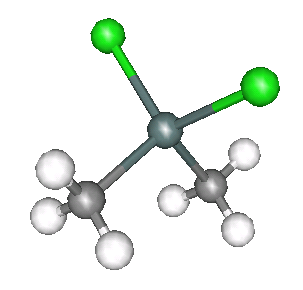
\includegraphics[width=0.5\linewidth]{../noxtal/images/dimethyltin_dichloride.png}\\
      Dimethyl tin dichloride
      \end{center}
    \end{column}
    \begin{column}{0.5\linewidth}
      \begin{center}
        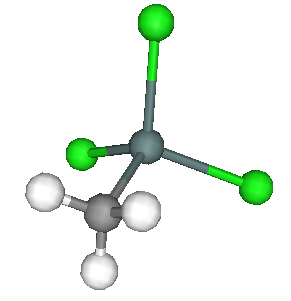
\includegraphics[width=0.5\linewidth]{../noxtal/images/monomethyltin_trichloride.png}\\
        Monomethyl tin trichloride
      \end{center}
    \end{column}
  \end{columns}
  \begin{columns}
    \begin{column}{0.33\linewidth}
      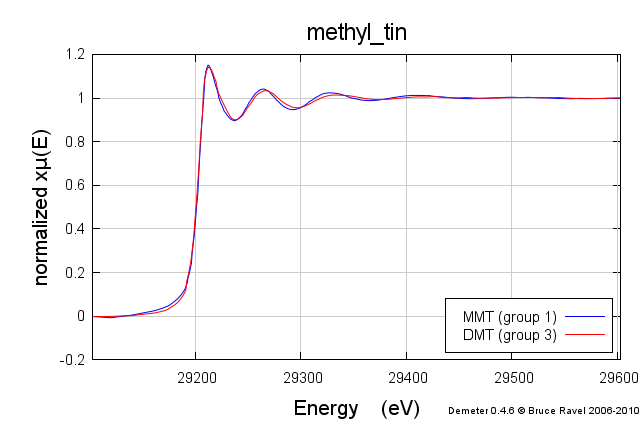
\includegraphics[width=\linewidth]{../noxtal/images/mtin_mu.png}
    \end{column}
    \begin{column}{0.33\linewidth}
      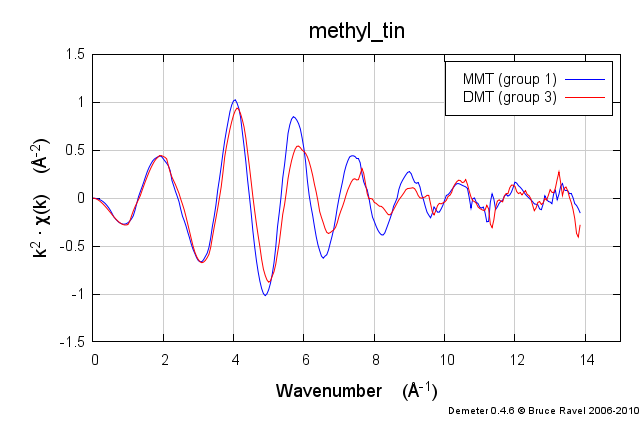
\includegraphics[width=\linewidth]{../noxtal/images/mtin_chik.png}
    \end{column}
    \begin{column}{0.33\linewidth}
      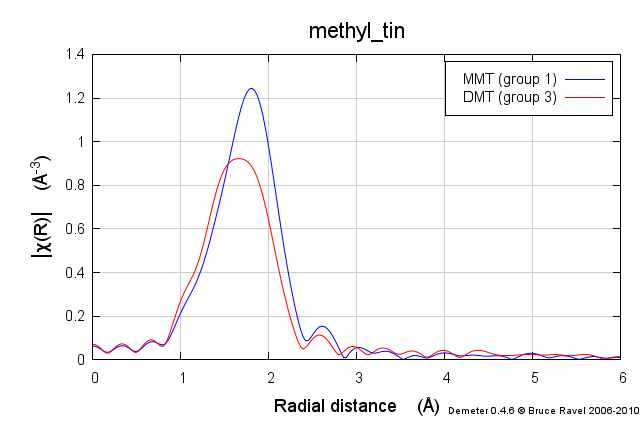
\includegraphics[width=\linewidth]{../noxtal/images/mtin_chir.png}
    \end{column}
  \end{columns}
\end{frame}


\begin{frame}[fragile]
  \frametitle{Protein Data Bank file format}
  A bit of googling turned up a structure for dimethyl tin dichloride
  in the form of a PDB file.  It looks like this:

  \begin{block}{}
\begin{alltt}
\scriptsize
COMPND    5261536
HETATM    1 \alert{ C}1  LIG     1      \alert{-0.027   2.146   0.014}  1.00  0.00
HETATM    2 \alert{SN}2  LIG     1      \alert{ 0.002  -0.004   0.002}  1.00  0.00
HETATM    3 \alert{ C}3  LIG     1      \alert{ 1.042  -0.716   1.744}  1.00  0.00
HETATM    4 \alert{CL}4  LIG     1      \alert{-2.212  -0.821   0.019}  1.00  0.00
HETATM    5 \alert{CL}5  LIG     1      \alert{ 1.107  -0.765  -1.940}  1.00  0.00
HETATM    6 1\alert{H}1  LIG     1      \alert{ 0.996   2.523   0.006}  1.00  0.00
HETATM    7 2\alert{H}1  LIG     1      \alert{-0.554   2.507  -0.869}  1.00  0.00
HETATM    8 3\alert{H}1  LIG     1      \alert{-0.537   2.497   0.911}  1.00  0.00
HETATM    9 1\alert{H}3  LIG     1      \alert{ 0.532  -0.365   2.641}  1.00  0.00
HETATM   10 2\alert{H}3  LIG     1      \alert{ 1.057  -1.806   1.738}  1.00  0.00
HETATM   11 3\alert{H}3  LIG     1      \alert{ 2.065  -0.339   1.736}  1.00  0.00
END
\end{alltt}
  \end{block}

The \alert{red bits} are atomic species and cartesian coordinates ---
just what we need!
\end{frame}

\begin{frame}[fragile]
  \frametitle{Feff6 input file}
  \begin{columns}
    \begin{column}{0.45\linewidth}
\begin{alltt}
\scriptsize
 {\color{Green4}TITLE dimethyltin dichloride}
 {\color{Purple2}HOLE}      1   1.0  {\color{Blue4} *  Sn K edge (29200 eV), S0^2}
 {\color{Blue4}*         mphase,mpath,mfeff,mchi}
 {\color{SteelBlue2}CONTROL}   1      1     1     1
 {\color{SteelBlue2}PRINT}     1      0     0     0
 {\color{Purple2}RMAX}      6.0

 {\color{Brown4}POTENTIALS}
 {\color{Blue4}*    ipot   Z  element}
        0   50   Sn        
        1   17   Cl
        2    6   C
        3    1   H
 {\color{Brown4}ATOMS}
 {\color{Blue4}*   x       y       z    ipot}
   -0.027   2.146   0.014  2
    0.002  -0.004   0.002  0
    1.042  -0.716   1.744  2
   -2.212  -0.821   0.019  1
    1.107  -0.765  -1.940  1
    0.996   2.523   0.006  3
   -0.554   2.507  -0.869  3
   -0.537   2.497   0.911  3
    0.532  -0.365   2.641  3
    1.057  -1.806   1.738  3
    2.065  -0.339   1.736  3
\end{alltt}      
    \end{column}
    \begin{column}{0.55\linewidth}
      ~\\[2ex]

      \begin{enumerate}
      \item Prepare \file{feff.inp} boilerplate
      \item Cut-n-paste the cartesian coordinates in the
        {\color{Brown4}\texttt{ATOMS}} list
      \item Make a {\color{Brown4}\texttt{POTENTIALS}} list out the
        atomic species
      \item The absorber \textbf{must} be potential \#0, but it need
        be neither first in the {\color{Brown4}\texttt{ATOMS}} list
        nor be at (0,0,0)
      \item The {\color{Brown4}\texttt{ATOMS}} list need not be in
        order of radial distance (or any other order)
      \item This \file{feff.inp} file can be imported directly into
        {\artemis}
      \end{enumerate}
    \end{column}
  \end{columns}
\end{frame}


\section{Simple fitting model}

\begin{frame}
  \frametitle{Create a simple fitting model}
  \footnotesize%
  \begin{enumerate}
  \item Import the dimethytin dichloride (DMT) data from the {\athena}
    project file
  \item Import the \file{feff.inp} file for DMT
  \item Run {\feff} then drag and drop the first two paths
    (Sn$\leftrightarrows$C and Sn$\leftrightarrows$Cl) onto the
    DMT data.
  \item Create guess parameters for an overall amplitude and an
    overall E$_0$ shift.
  \item We cannot expect to share $\sigma^2$ or $\Delta R$ 
    between the C and Cl scatterers, so create 4 more parameters for
    those.  That's \alert{6} guess parameters.
  \item With the k-range set to [2:10.5] and the R-range set to
    [1:2.4], we have at most about \alert{7.5} independent points.
  \end{enumerate}
  \begin{columns}
    \begin{column}{0.4\linewidth}
      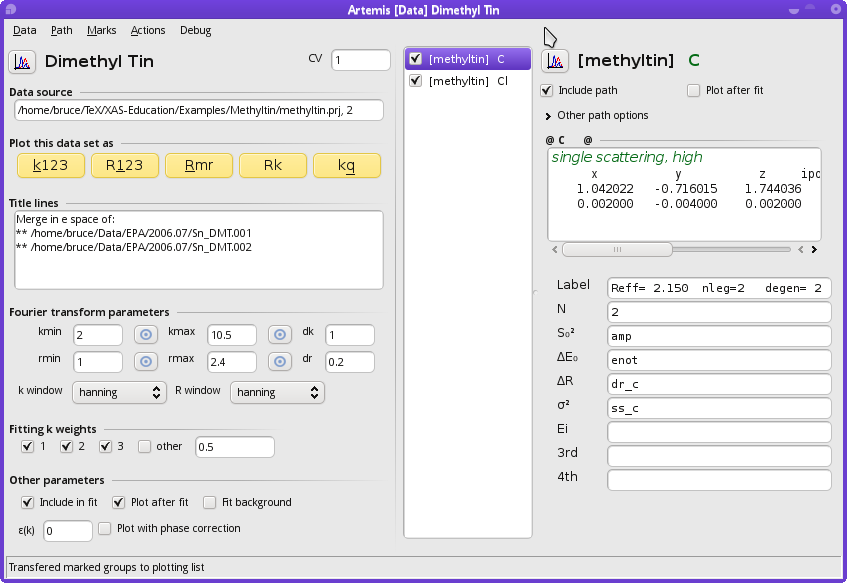
\includegraphics[width=\linewidth]{images/dmt_start.png}      
    \end{column}
    \begin{column}{0.6\linewidth}
      Guess 1 for the amplitude, 0 for both $\Delta R$ parameters and
      0.003 for both $\sigma^2$ parameters.
    \end{column}
  \end{columns}
\end{frame}

\begin{frame}[fragile]
  \frametitle{Results of the first fit}
  \small
  The fit doesn't seem bad.  The {\color{Red3}red line} overplots the
  {\color{Blue3}blue line} rather well.  Unfortunately, the amplitude
  and both $\sigma^2$ parameters are suspiciously large, and one
  correlation is quite alarming.
  \begin{columns}
    \begin{column}{0.5\linewidth}
      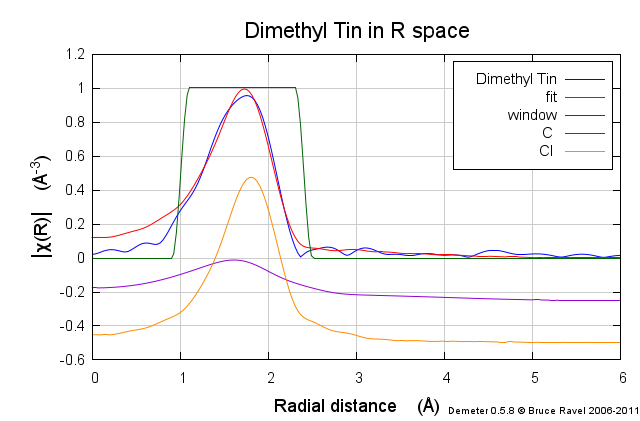
\includegraphics[width=\linewidth]{images/dmt_kw2_fit.png}
    \end{column}
    \begin{column}{0.5\linewidth}
\begin{alltt}
\tiny 
\alert{Independent points          : 7.426757813
Number of variables         : 6}
Chi-square                  : 3016.609652735
Reduced chi-square          : 2114.310940726
R-factor                    : 0.007830860
         
guess parameters:
  \alert{amp           =   3.17612332    # +/-   1.20737984}
  enot          =   5.48632866    # +/-   3.83329304
  dr_c          =   0.15998621    # +/-   0.10183822
  dr_cl         =   0.00886040    # +/-   0.02941155
  \alert{ss_c          =   0.04405173    # +/-   0.02749584}
  \alert{ss_cl         =   0.01784104    # +/-   0.00499746}

Correlations between variables:
          \alert{ss_cl & amp            -->  0.9231}
          dr_cl & enot           -->  0.8694
           dr_c & amp            -->  0.7677
           ss_c & enot           --> -0.6554
          ss_cl & dr_c           -->  0.6873
           ss_c & amp            -->  0.6070   

\end{alltt}
    \end{column}
  \end{columns}
  These data are severely stressed by fitting 6 parameters with barely
  more information.  That is the likely cause of the odd results.

  \medskip

  Now, click the buttons for k-weighting by 1 and 3 in the fit.
  Re-run the fit.
\end{frame}

\begin{frame}[fragile]
  \frametitle{An unstable fit}
  \small
  There is an even worse aspect of the fit we just did.  It turns out
  that it is very unstable.  The result we just found is some kind of
  local minimum, but perhaps not the best fit.
  \begin{columns}
    \begin{column}{0.5\linewidth}
      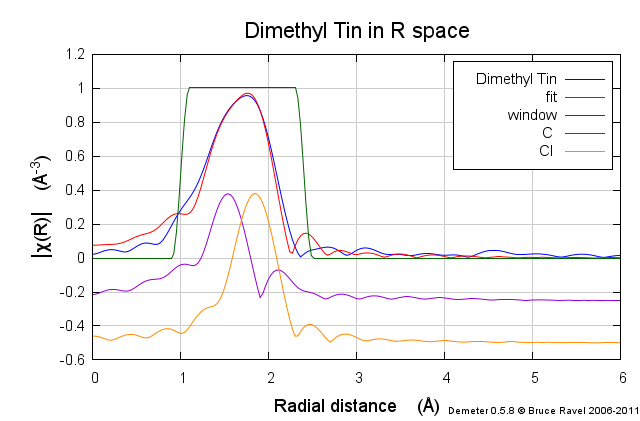
\includegraphics[width=\linewidth]{images/dmt_better.png}      
    \end{column}
    \begin{column}{0.5\linewidth}
\begin{alltt}
\tiny
\alert{Independent points          : 7.426757813
Number of variables         : 6}
Chi-square                  : 16890.423023572
Reduced chi-square          : 11838.325240341
R-factor                    : 0.016206958

guess parameters:
  {\color{Green4}amp           =   1.19951643    # +/-   0.27919514}
  enot          =   3.72054447    # +/-   2.58474466
  dr_c          =  -0.06264818    # +/-   0.04220613
  dr_cl         =   0.01464366    # +/-   0.02710054
  {\color{Green4}ss_c          =   0.00208373    # +/-   0.00627642
  ss_cl         =   0.00506975    # +/-   0.00429784}

Correlations between variables:
          dr_cl & enot          -->  0.8889
          ss_cl & ss_c          -->  0.8785
          ss_cl & amp           -->  0.8698
           dr_c & enot          -->  0.8547
           ss_c & amp           -->  0.8429
          dr_cl & dr_c          -->  0.8047

\end{alltt}
    \end{column}
  \end{columns}
  This is an improvement in that the amplitude and the $\sigma^2$
  values are much more in line with what we expect, but correlations
  remain quite high.

  \medskip

  The next trick to try is a multiple data set fit.
\end{frame}

\section{Multiple data set fit}


\begin{frame}
  \frametitle{Setting up a multiple data set fit}
  Import the monomethyl tin trichloride (MMT) from the {\athena}
  project file.  This will open a second Data window and place a
  second item in the list of data sets.
  \begin{center}
    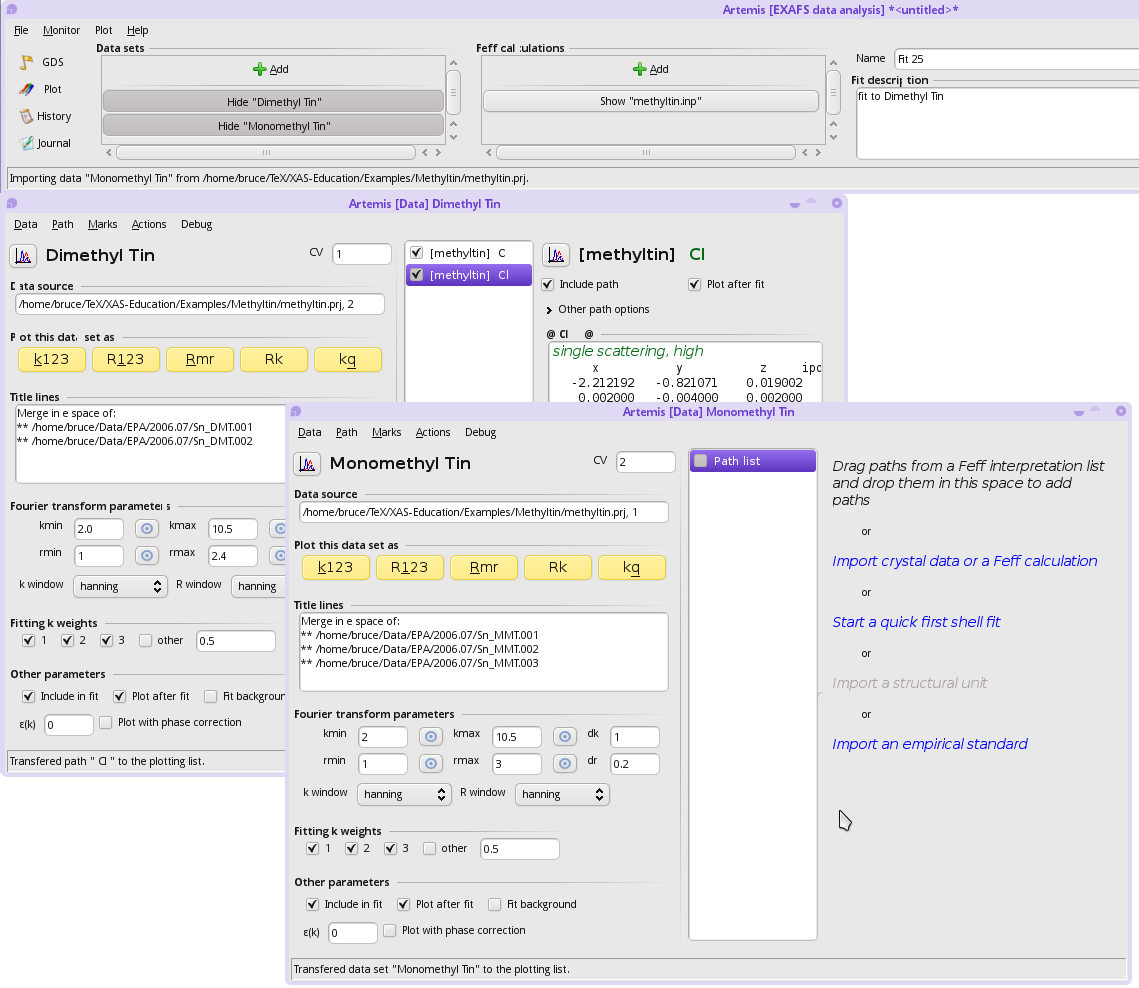
\includegraphics[width=0.7\linewidth]{images/mds.png}
  \end{center}
\end{frame}

\begin{frame}
  \frametitle{Cloning paths from DMT to MMT}
  \small
  Drag and drop both paths from the DMT window to the MMT window.
  Path drag and drop works by clicking on a path in the path list of
  the source \textit{while holding down the control key}.

  \begin{center}
    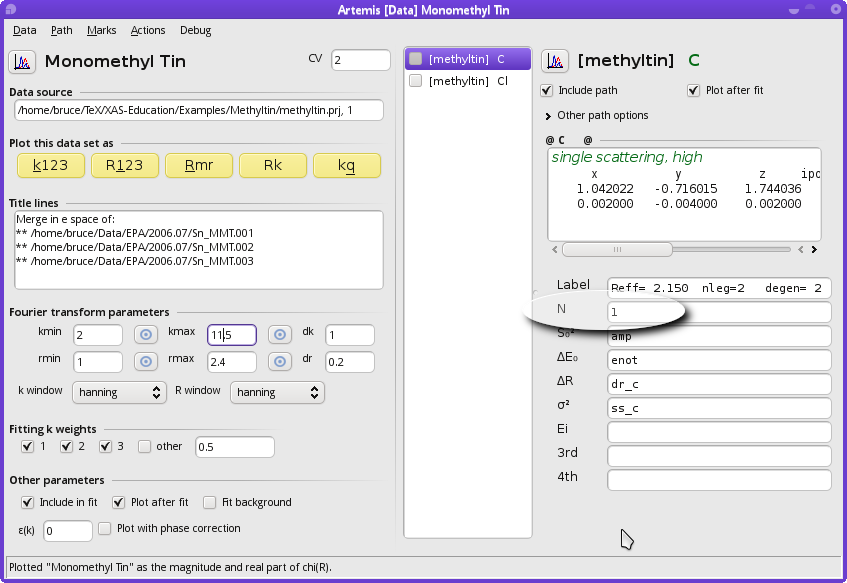
\includegraphics[width=0.65\linewidth]{images/MMT.png}
  \end{center}
  
  Change the N of the Sn$\leftrightarrows$C path to 1, since
  monomethyl tin only has one methyl ligand.  Similarly, change the N
  of the Sn$\leftrightarrows$Cl path to 3, since there are three Cl ligands.
\end{frame}

\newtheorem{assumption}[theorem]{Assumption}

\begin{frame}
  \frametitle{Discussion}
  \begin{assumption}
    The Sn--C and Sn--Cl bonds are identical in DMT and MMT, thus we
    can use the same $\sigma^2$ and $\Delta R$ parameters for each
    data set.
  \end{assumption}

  Given this assumption, the fitting situation is much improved.  We
  have \alert{doubled} the information content while introducing
  \alert{0} additional parameters!

  \begin{columns}
    \begin{column}{0.5\linewidth}
      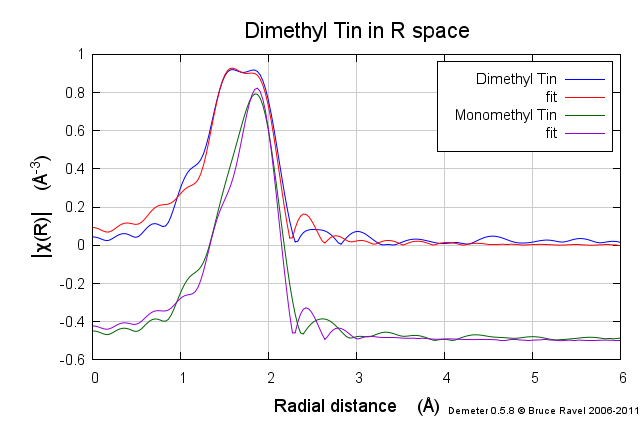
\includegraphics[width=\linewidth]{images/MDS_fit.png}
    \end{column}
    \begin{column}{0.5\linewidth}
      The best fit values are much the same as for the better single
      data set fit.  The fit, however, is more stable and independent
      of the starting values.  The correlations are mostly smaller.
    \end{column}
  \end{columns}
\end{frame}

\begin{frame}
  \frametitle{What's next?}
  \begin{enumerate}
  \item Could the Fourier transform range be longer?  Look at the k123
    plot for each data set.
  \item Is the assumption about the bonds in the two samples valid?
    How would you go about testing the assumption?
  \item Trimethyl tin monochloride would have been useful to
    measure....
  \item The $\Delta R$s for both Sn$\leftrightarrows$C and the
    Sn$\leftrightarrows$Cl are rather large.  The fit might be
    improved by adjusting the original \file{feff.inp}, re-running
    {\feff}, and re-doing the fit.
  \end{enumerate}
\end{frame}
\end{document}


%%% Local Variables:
%%% TeX-parse-self: t
%%% TeX-auto-save: t
%%% TeX-auto-untabify: t
%%% TeX-PDF-mode: t
%%% End:
